\subsection{PsychSim}
\label{sec:psychsim}
\begin{figure}
  \centering
    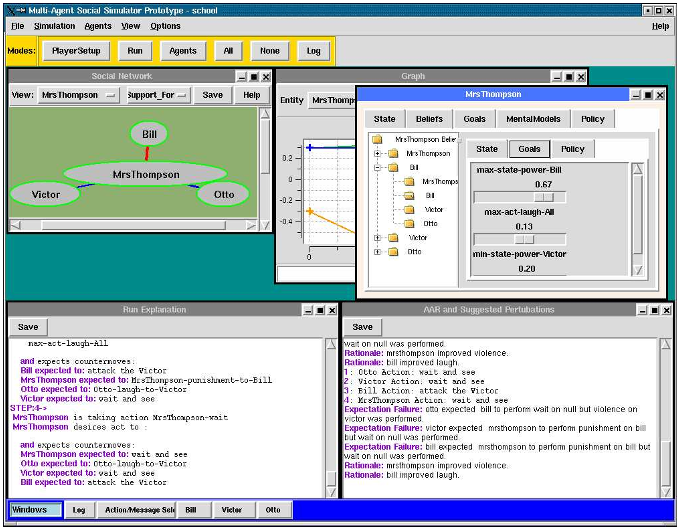
\includegraphics[width=.7\textwidth]{psychsim}
  \caption{PsychSim tool for generating new scenarios and agents.}
  \label{fig:psychsim}
\end{figure}
PsychSim \cite{marsella:psychsim} is a social simulation tool developed to explore how individuals and groups interact and how can these interactions be influenced.
The work's foundation is the fact that social interactions are based on beliefs about other's minds, a \textit{theory of mind} \cite{whiten:theoryofmind}.
Psychsim allow the users to author and explore a social scenario of his creation through the selection of generic agents models and its further specialization, see Fig. \ref{fig:psychsim}.
This tool allows users to try and understand how a specific social group might react to certain situations.

PsychSim then simulates the behaviour for each entity, individual agent or group of agents, based on their preferences, relationships, private beliefs, and mental models about each other.

In the given example, the authors explore a bullying scenario in a school and try to answer several questions:
"\textit{How might a bully respond to admonishments, appeals to kindness or punishment? 
How might other groups react in turn? 
What are the predictions or unintended side effects?}".
The simulation tool then provides explanations of the results based on each entity's preferences and beliefs, allowing the user to answer the previous questions.

PsychSim's agents are empowered with fully specified models of each other \cite{pynadath:modellingtheoryofmind}, a unique aspect of its design. Every agents maintains independent beliefs about the world, has its own goals, and it owns policies to achieve those goals. The model is composed by the state, actions, goals, beliefs, policies, messages, and mental models.

\begin{description}
\item \textbf{State} Each agent model includes a state with facts about the world, some of which may be hidden from the agent.
\item \textbf{Actions} Agents have a set of actions they can perform. Each action consists in an action type, a performer, and possibly an object of the action.
\item \textbf{Goals} These represent an agent's incentives for behaviours. In PsychSim, goals are reward functions that map the current state to a real value.
\item \textbf{Beliefs} The simulations agent have only a \textit{subjective} view of the world, where they form beliefs about what \textit{they} think is the state of the world. An agent's beliefs consists in models of all agents (including himself), representing their state, beliefs, goals, and policy of behaviour.
\item \textbf{Policies} Each agent's policy is a function that represents the process by which it selects an action or message based on its beliefs and goals.
\item \textbf{Messages} Messages are attempts by one agent to influence the beliefs of recipients and have five components: a source, recipients, a message subject, content, and overhearers.
\item \textbf{Mental Models} An agent's beliefs about another agent are realized as a fully specified agent model of the other agent, including goals, beliefs, and policies. Mental Models are predefined models which represent agents goals, beliefs, and policies.
\end{description}

As a social agent architecture, PsychSim presents a well-defined model capable of fully simulating social behaviour.
It is based on sound theories from psychology (theory of mind) and has into account other agents in its cognitive process, a requirement for social agents as we saw in \ref{sec:social-agents}.

However, PsychSim lacks planning capabilities.
Based only of policies to guide it's immediate behaviour, each agent will follow the scenario devised by the user disregarding any future states.